%# -*- coding: utf-8-unix -*-
%%==================================================
%% 02_dpa.tex % 4.5k
%%==================================================

\chapter{功耗分析攻击}
在之前一章,我们提到了很多种旁路攻击的手段。其中功耗分析攻击是被研究最多的一种,其应用也最广。

功耗分析攻击所需的花费极低,即使是普通的采集设备和示波器,辅以简单的软件程序,就能完成攻击。与此同时,功耗分析攻击不会对设备进行拆解动作,因此不会留下破坏的痕迹,也不会损伤设备,这既降低了研究的成本,也减少了攻击被发现的可能性。

因此,作为旁路攻击的一种最为典型的方法,我们有必要详细研究这种方法。研究清楚了功耗分析攻击,再去研究其他类型的攻击方式就要容易多了。

\section{功耗构成}  % 0.5k
我们在前面提到过,密码设备通常是由数字电路构成的,而数字电路的基本元件采用的是 CMOS 工艺。因此设备的功耗也就是整个 CMOS 构成的数字电路的功耗,要研究密码设备的功耗,就需要研究 CMOS 电路的功耗来源和组成。

我们这里所说的功耗,通常是指整个设备的产生的总功耗,一般采集到的也都是这类功耗。

逻辑元件的功耗一般分为静态功耗和动态功耗。

静态功耗通常来自于晶体管的漏电流,其占比相对较低,不过需要注意的是,随着单个晶体管的尺寸越来越小,漏电流的比重在逐渐提高。当然,在实际的攻击中,静态功耗基本可以忽略不计。

动态功耗通常来自信号的翻转,从而造成晶体管的截断或者导通,此时等价于电流对晶体管的本征电容和寄生电容进行充放电。另一部分动态功耗来自瞬时的短路电流。还有一种需要考虑的情况是电路工作时产生的毛刺,这类毛刺往往会产生很高的瞬时功耗,而且和数据相关,因此需要特别关注。总之,动态功耗一般是元件功耗的主要组成部分,我们通常采集的功耗,也大多数是动态功耗。


\section{功耗仿真}  % 1k
在数字电路的设计阶段,设计者往往要对电路产生的功耗进行仿真。一方面是为了尽可能降低电路的功耗,以提高电路的市场竞争力;另一方面是为了避免出现较为明显的毛刺之类不利因素,影响电路的基本功能;还有一方面就是出于安全方面的考虑,尽可能地减少功耗泄露的信息。

我们可以在不同的层级对电路的功耗进行仿真。仿真的级别越底层,粒度越细,仿真的结果就有可能越符合实际情况,当然也就需要消耗更多的计算资源;相反,仿真的级别越高层,粒度越粗,仿真的结果出现偏差的可能性就越高,不过带来的好处就是较少的计算资源和仿真时间。所以具体选择在哪个层级对电路的功耗进行仿真,需要视具体情况而定,在成本和拟真度之间做一个较好的折中。

功耗仿真的层级按照粒度从粗到细,可以分为行为级、逻辑级和模拟级。

对电路功耗最为粗糙的仿真,就是行为级的仿真。行为级的仿真通常只考虑电路的重要组成部件,比如控制单元、处理单元、存储单元以及专门的运算单元。行为级仿真通常在数据的操作或者程序的运行这一层面考虑问题,这是因为设备的功耗往往是依赖于操作的数据和运行的程序的。尽管行为级的仿真可能无法给出非常精确的结果,但是较高的仿真速度可以让开发人员在设计初期就能迅速对电路的功耗有一个大致的感觉,从而更好地指导后续的电路设计。

稍细粒度的功耗仿真是逻辑级仿真。数字电路设计软件可以在设计者画出电路的同时,生成电路的网表,这些网表表示电路中各个逻辑元件之间的连接关系,以及一些相关的参数和信息,比如信号的上升和下降延时。在这一层级,仿真通常会用到汉明距离模型或者汉明重量模型,这两类模型对功耗进行了简化,以此降低计算的复杂度,提高仿真的速度。

模拟级的功耗仿真是粒度最细的,得到的仿真结果也是三种当中最为精确的,当然也就意味着耗费的时间和成本最高。电路的各种连接关系以及详细的参数都记录在晶体管网表中,寄生电容这类实际出现的效应也会被纳入计算。然而,由于晶体管数目极为庞大,如果将所有参数都考虑进来,计算耗费的时间和成本将十分可观。因此仿真时往往会对电路的模型做一些必要的简化,这会带来一定的精度损失。所以,需要在精度和速度之间做一个折中。一般不会对整个电路做模拟级的仿真,因为这样付出的代价实在太大。只有对重要的和关键的部件才会进行模拟级的仿真,因为得到这些部分的功耗信息可能比其他部分更加有用,或者更有参考价值。

\section{功耗采集} % 1k
\label{sec:collect}
即使采用了最好的功耗模型,选取了最细的仿真粒度,仿真得到的结果有可能依旧和实际情况相去甚远。而且功耗仿真一般在设计阶段,设计者拥有较多的关于电路的参数和信息。而攻击者几乎不掌握设备的基本信息,也就无从对电路建立功耗模型,当然也就无从对电路的功耗进行仿真。所以,对于攻击者而言,最切实可行的做法就是直接在设备运行时采集到实际的功耗。而若要采集设备的功耗,就必须配置好相关的仪器,因此我们下面介绍一下采集电路功耗要做的准备工作。

\vspace*{\baselineskip}

下面列举一些采集功耗所需的基本的仪器和装置:

\begin{itemize}
\item \textbf{被攻击的密码设备:}研究人员需要将密码设备中输入输出的接口连接到对应的采集设备和分析装置上。
\item \textbf{电源与适配器:}不同的密码设备所需的供电电压与工作条件不尽相同,研究人员需要根据具体的设备提供合适的电源和适配器,以保证密码设备的正常工作,从而得到正常的有效的功耗。
\item \textbf{时钟信号发生装置:}要让密码设备稳定的工作,就需要收到稳定的时钟信号,因此良好的时钟信号发生装置必不可少。如果有特殊的要求,研究人员还需要自己制作特定的时钟发生电路。
\item \textbf{功耗捕捉装置:}电路的功耗很难直接测得,往往体现在某些具体的信号数值上,比如供电电源线上的总电流或者测量电阻上的电压。因此,若要得到电流,就需要将测量电路接在供电装置与密码设备之间。一个比较简单的测量电路就是串接合适大小的电阻。当然,除了插入测量电路之外,也可以使用电磁探针,通过采集电磁信息,间接地得到功耗数据。总之,功耗捕捉装置可以采用不同的方案,视具体的要求和成本而定,选取合适的即可。
\item \textbf{示波器:}从功耗捕捉装置中得到的信号(电压、电流、磁场)需要通过示波器来采集、呈现和记录。在功耗分析攻击中,普通的数字示波器即可满足要求。不过选取合适的示波器仍然需要考虑一些具体的参数,比如示波器的采样率、带宽以及分辨率,这个同功耗捕捉装置一样,根据具体的情况选取合适的配置。
\item \textbf{计算机:}计算机的作用在于控制整套功耗采集的设备,并将采集的信息储存下来,用于后续的分析和处理。因此研究人员需要能够保证密码设备、功耗捕捉装置、示波器以及计算机之间的正常通信,这个有时候是一个并不简单的任务。

\end{itemize}

\vspace*{\baselineskip}

功耗采集的流程如下:

\begin{enumerate}
\item 开启密码设备、示波器以及计算机,并且保证均可正常工作和有效通信;
\item 计算机向密码设备发送特定的指令使其正常工作,运行设备内部的程序;
\item 与此同时,功耗捕捉装置产生电流、电压或者磁场信号,并通过示波器呈现和采集;
\item 计算机获取密码设备的返回数据,并储存示波器采集的功耗数据;
\item 不断重复上述过程,直到采集的功耗数据量满足研究人员的需要。

\end{enumerate}


\section{差分功耗分析} % 1.5k
\label{sec:dpa}
功耗分析通常包含简单功耗分析(Simple Power Analysis)和差分功耗分析(Differential Power Analysis)。

简单功耗分析通常只需要少量的功耗曲线,就能揭示密码设备中的有用信息。简单功耗分析通常适用于功耗曲线特征较为明显的密码设备,比如出现明显的波峰和波谷,以及呈现出多个周期性的重复段落。如果攻击者对密码设备中运行的程序有一定的预备知识,那么就能推测出功耗曲线的不同段落在执行何种操作,就有可能进一步掌握设备的更多信息。

差分功耗分析则需要大量的功耗迹。大量功耗数据带来的好处就是更强大的分析和攻击能力,也不需要对设备的构造和执行的程序有详细的了解,一般情况下,只要掌握设备运行的算法流程就足够实施分析和攻击了。

因此,我们的关注重点就放在差分功耗分析上。

\vspace*{\baselineskip}

下面我们来介绍一下差分功耗分析的一般流程:

\begin{enumerate}
\item \textbf{选取合适的算法中间值位置:}一个好的中间值,应该尽可能地区错误的猜测和正确的猜测。因此,在密码算法中,通常选择非线性函数的输出作为差分功耗分析的中间值。由于在运行算法和采集功耗时,攻击者往往只能获得明文或者密文,因此通常只能对算法的第一轮加密或者最后一轮加密进行攻击。因此,选取的中间值最好能够出现在第一轮或者的最后一轮。选取不同的中间值,会对攻击效果产生很大的影响,因此需要根据不同的算法和具体的实验条件,选取最合适的算法中间值。
\item \textbf{采集设备运行时的实际功耗曲线:}这一部分没有什么技术难度,不过值得一提的是,如果合理地选择功耗曲线采集和结束的位置,就能得到对齐较好的曲线,方便后续的分析和处理。采集环境也要尽可能地排除外界因素的干扰,以提高功耗曲线同数据和操作的相关性,增大信号的信噪比。更多具体的细节已经在上一小节阐述了。
\item \textbf{根据算法计算理论中间值:}对某个具体的密码算法而言,密钥通常是最重要也是最机密的信息,攻击者唯一无法知晓的也是这一部分。对全部位数的密钥进行穷举猜测是不可能做到的,因此攻击者常常需要在选择合适的中间值的前提下,尽可能地降低中间值和全部密钥之间的相关性。或者说,攻击者应该尽可能选取只依赖少部分密钥的中间值,这样就能大大减少猜测的可能情况,提高攻击的效率。由于密码算法通常是公开透明的,因此已知明文和猜测密钥的情况下,是可以计算出适合的理论中间值的。
\item \textbf{使用合适的功耗模型将理论中间值转换为假设功耗值:}算法的中间值通常是某个字节或者比特,和算法有关。由于中间值的值域很大,因此对所有可能的中间值建立一个具体的模型是不现实的。所以有必要采用合适的功耗模型,缩小猜测空间,将中间值转换成假设功耗值。常用的功耗模型包括汉明重量模型、汉明距离模型以及零值模型。功耗模型之间各有利弊,需要根据实际的实验情况和攻击效果选取最合适的模型。
\item \textbf{分析假设功耗值和实际功耗曲线,挖掘所需的信息:}这部分通常涉及到一定的统计学知识,需要攻击者具备较好的数学基础。在分析曲线的特征之前,通常还要对功耗曲线进行预处理,比如对齐和滤波,减少噪声,提高信噪比,从而能够更好地利用功耗曲线中的有效信息。此外,高效地处理大量的数据也是一个需要仔细考量的问题,差分功耗分析往往会采集成千上万甚至是百万条曲线,如何编写性能优异的算法,或者是并行化处理,都会很大程度上影响分析的速度和效果。除了常用的相关系数攻击之外,模板攻击也很有效。攻击者应该尽可能地设计好的算法,从而减少所需的功耗曲线条数,这样就能大大减少攻击的时间和成本。
\end{enumerate}

\vspace*{\baselineskip}

图 \ref{fig:dpa} 展示了差分功耗分析攻击的第 3 -- 5 步。

\begin{figure}[htbp]

    \centering
    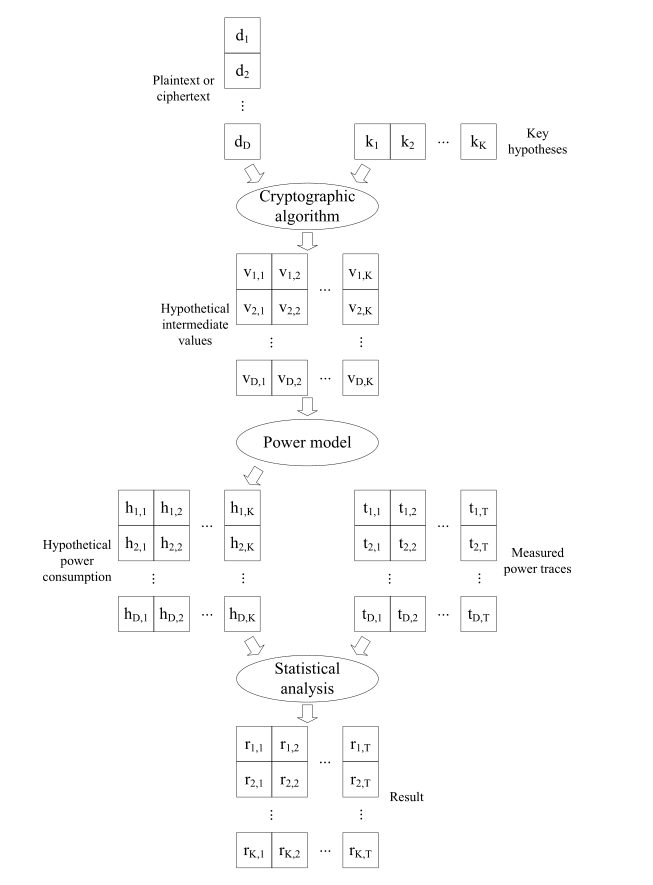
\includegraphics[height=.8\textheight]{../images/dpa.png}
    \caption{差分功耗分析的典型流程}
    \label{fig:dpa}
\end{figure}